% !TEX encoding = UTF-8
% !TEX TS-program = pdflatex
% !TEX root = ../tesi.tex

%**************************************************************
\chapter{Analysis and design of Stipula platform}
\label{cap:general-design}
%**************************************************************.

This chapter provides a possible design for the implementation of the \textit{Stipula} language. In 
particular, the general architecture of the implementation will be illustrated, with its components and 
modules. Furthermore, the various design choices will be explained and justified.
%**************************************************************

\section{Blockchain layers}
\label{blockchain-layers}

Over the years, blockchains such as those of Bitcoin and Ethereum have established themselves in the new 
distributed context. One problem that has arisen and is recognized is the \textit{scalability issue} of 
these solutions. Blockchains like the ones mentioned fail to scale much when faced with having to process a 
large amount of transactions. Furthermore, this amount of transactions can congest the network of 
blockchain nodes and increase fees for logging information into the ledger. Therefore, over the years, 
solutions have been designed and implemented that could remedy the problem of scalability. These new 
solutions use an \textit{underlying blockchain as a basis}, such as Bitcoin and Ethereum, and develop 
solutions that allow for an increase in transaction throughput, while trying to keep the cost of 
commissions low. To do this, scalability solutions need a secure and decentralized layer. Networks such as 
Bitcoin and Ethereum are defined as \textbf{layer one}, that is, they represent the fundamental layer on 
which it is then possible to build other applications, while scalability solutions are defined as 
\textbf{layer two}.

There are mainly four types of layer two:
\begin{enumerate}
	\item \textit{Nested blockchain} (i.e., Plasma, \cite{site:plasma-ethereum}): they run on top of another 
	(i.e., Ethereum). Layer one establishes the settings and layer two conducts the procedures;
	\item \textit{Sidechains} (i.e., Polygon, \cite{site:polygon-ethereum}): delegate massive transactions, 
	but this kind of chain is less integrated into the core blockchain. They can have a different consensus 
	algorithm from the blockchain layer one;
	\item \textit{Rollups} (i.e., Arbitrum, \cite{site:arbitrum}, and Optimism, \cite{site:optimism}): the 
	transactions are computed off-chain but the data are saved on the blockchain layer one;
	\item \textit{State channels} (i.e., LightningNetwork, \cite{site:lightning-network}): establish two-way 
	communication between a blockchain layer one and off-chain channels. The transactions are saved on the 
	blockchain layer one when they will be completed on the state channel.
\end{enumerate}
The first three solutions use a dedicated ledger in layer two similar to that of layer one. Instead, state 
channels use other cryptographic methods and ad-hoc communication protocols, without the need to have 
their own ledger in which to store the information. Only a minimal amount of information, produced by this 
type of scalability solution, is stored in the underlying layer one.

This separation between layers allows:
\begin{enumerate}
	\item Layer one to focus on network and ledger distribution and security;
	\item Layer two to focus on \textit{scaling} transaction processing.
\end{enumerate}

\section{Basic ideas}
\label{basic-ideas}
As stated in the dedicated chapter, it was possible to notice how the \textit{Stipula} language offers 
peculiar functions compared to the other languages present in the smart contract environment. In particular, 
it has been possible to find that the language requires that the concept of time is not dependent on 
external factors, such as the time required for the generation of a block. Furthermore, the functionality 
of invoking events scheduled over time is such that it must be managed ad-hoc in the implementation, and 
that currently there is no similar one in the various languages for smart contracts, except by resorting to 
the use of software external to the system (i.e., oracles). Therefore, due to these particular 
functionalities that must be guaranteed by the language, one of the ideas behind the realization of the 
project is to provide an implementation of the language as a dedicated \textit{layer} which rests on 
another underlying layer. With this concept we want to place a marked separation between the layer that 
deals with saving information in an immutable register and guaranteeing security, and the layer that deals 
with the execution of contracts. Thus subdivided, the lower layer is used as a \textit{commitment} state, 
where the upper layers use that layer to \textit{timestamp} the information; whereas, the layer that 
implements the \textit{Stipula} language only deals with the execution of contracts (i.e., contract 
status management, asset transfer management, \dots) and guarantees compliance with all the constraints 
imposed by the language , delegating information storage to the lower layer.

Another of the main ideas that guided the entire planning phase, and subsequently also the implementation 
phase, is the creation of a system that could be performed both in \textit{centralized} and in 
\textit{distributed} form. In fact, the implementation developed in this thesis work allows you to:
\begin{enumerate}
	\item Use it as a single instance on a server;
	\item Create a distributed network of \textit{nodes}. By node we mean an instance of the implementation 
	that is able to communicate with other instances of the same implementation to update itself regarding, 
	for example, the states of the contracts in execution. A network of nodes thus defined can be 
	centralized, that is, there is a single point of control that manages all aspects of the network (i.e., 
	updates, communications between nodes, \dots), or, \textit{decentralized}, that is, not there is a 
	central body that manages the network, but all the nodes are equal to each other (a \textit{peer-to-peer} 
	network). By doing so, a network of nodes providing a language implementation can be classified as a 
	layer one;
	\item Create a network of nodes that rely on an underlying layer (i.e., HyperLedger Fabric). It is also 
	possible to use layer two as a commitment layer. State channels (i.e. \textit{Lightning Network}) could 
	also be used for data commitment. However, the way they're designed doesn't make writing information as 
	easy as other scaling solutions (see section \ref{blockchain-layers}). Again, network management can be 
	centralized or decentralized.
\end{enumerate}

Throughout the thesis, reference will be made to \textbf{Stipula server} and \textbf{Stipula node}: 
\textit{server} means the instance of the language implementation running on a single machine. This mode 
mirrors the \textit{client-server} architecture, in which there is a machine that provides a service and 
some clients who want to take advantage of this offered service. By \textit{node}, on the other hand, we 
mean that the instance of the language implementation runs on different machines, which are able to 
communicate with each other to exchange information. Therefore, this architecture needs communication 
protocols and a layer that allows to manage the \textit{consent}. In particular:
\begin{enumerate}
	\item A \textit{Stipula server} is a application that runs in a single machine. It is able to execute 
	contracts and transfer assets among users. It does not have any module about consensus or module that 
	allows a communication with other \textit{Stipula servers};
	\item A \textit{Stipula node} is able to do all the things cited at the previous point, and it is able 
	to communicate with other \textit{peers} (other nodes), in order to exchange information about the 
	network and the consensus about contract states evolution.
\end{enumerate}

In the figure \ref{fig:differnte-configs} it is possible to notice the possible configurations that the 
designed architecture can support:
\begin{enumerate}
	\item It is possible to run \textit{Stipula server} on a single machine. This server has no way to 
	communicate with other servers and is suitable for a centralized concept;
	\item It is possible to run a \textit{Stipula server} and which uses a blockchain as an underlying layer. 
	The blockchain can be both layer one (\textbf{L1}) and layer two (\textbf{L2}) as long as it is possible 
	to record information in a ledger (therefore it is not possible to use state channels). All information 
	regarding contracts and asset transfers will also be stored in the underlying layer;
	\item It is possible to create a network of \textit{Stipula nodes}, which are able to communicate with 
	each other for the maintenance of the network itself and to exchange information regarding the consensus 
	of the results obtained from the execution of the contracts. There is no need for an underlying layer;
	\item To increase security, it is possible to extend the scenario described in the previous point and 
	also use a blockchain as a lower layer in which information regarding contracts and asset transfers can 
	be immutably stored.
\end{enumerate}

\label{fig:differnte-configs}
\begin{figure}[htbp]
	\centering
	\subfloat[Example of an instance of a \textit{Stipula} server.]
	{\label{fig:server-stipula}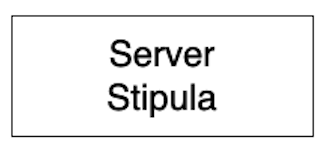
\includegraphics[width=0.3\textwidth]{immagini/capitolo-4/server-stipula.png}}
	\hspace{1cm}
	\subfloat[Example of an instance of a \textit{Stipula} server that relies on a blockchain.]
	{\label{fig:server-stipula-with-commitment}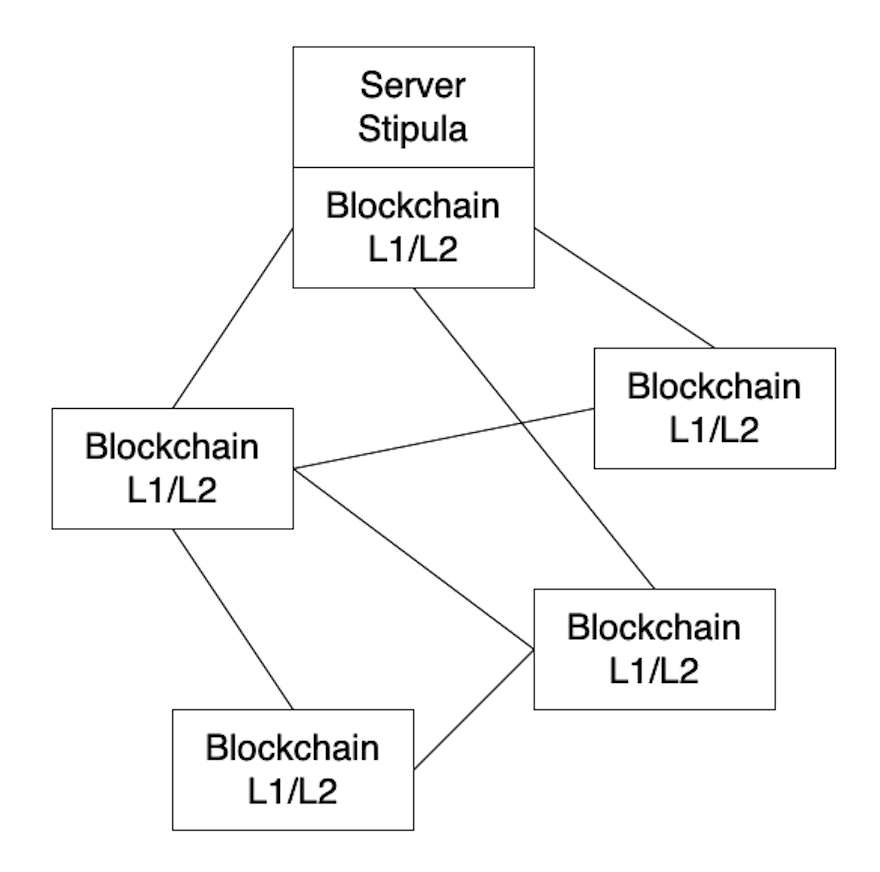
\includegraphics[width=0.4\textwidth]{immagini/capitolo-4/server-stipula-with-commitment.png}}\\
	\subfloat[Example of a network of \textit{Stipula} nodes.]
	{\label{fig:stipula-nodes}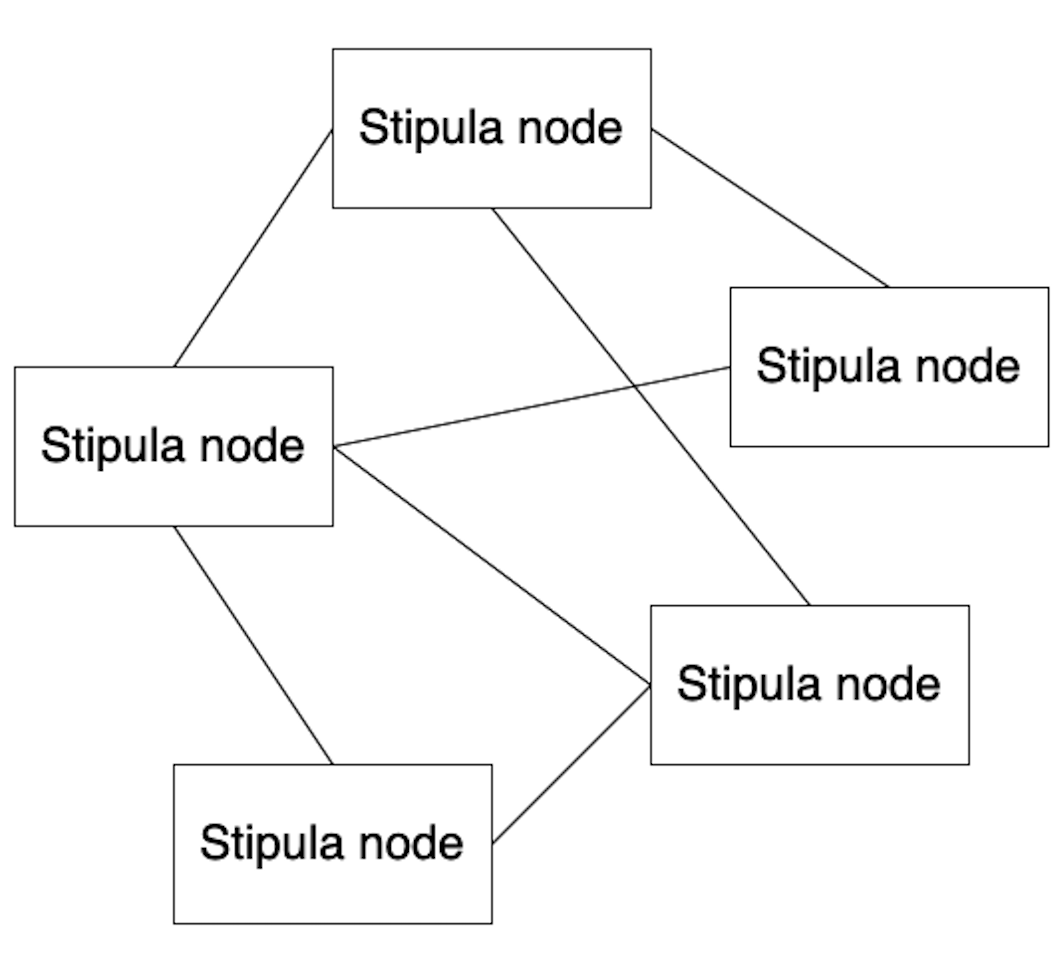
\includegraphics[width=0.4\textwidth]{immagini/capitolo-4/stipula-nodes.png}}
	\hspace{1cm}
	\subfloat[Example of a network of \textit{Stipula} nodes based on a blockchain.]
	{\label{fig:stipula-nodes-with-commitment}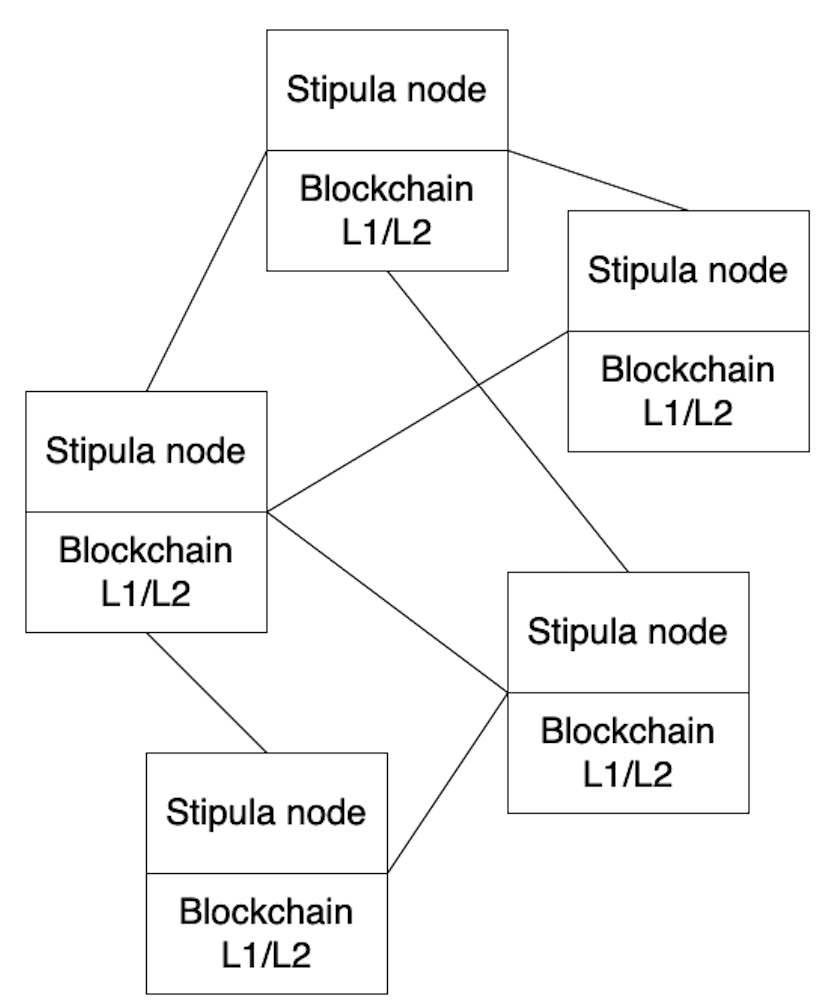
\includegraphics[width=0.4\textwidth]{immagini/capitolo-4/stipula-nodes-with-commitment.png}}
	\caption{Possible configurations of the \textit{Stipula} architecture.}
	\label{fig:network-configs}
\end{figure}

\newpage
\section{Architecture}

The main modules that make up the implementation architecture of the \textit{Stipula} language are
(\ref{fig:complete-architecture}):
\begin{enumerate}
	\item \textit{Message Service}: manages connection and communication with clients;
	\item \textit{Compiler}: receives as input a contract written in the \textit{Stipula} language and 
	compiles it in another language, called \textit{Stipula bytecode};
	\item \textit{Virtual Machine}: execute the code in \textit{Stipula bytecode} received as input;
	\item \textit{Consensus}: implements mechanisms that make it possible to determine consensus regarding the 
	result of executing a contract, within a network of nodes;
	\item \textit{Storage}: stores information about \textit{assets} and its \textit{transfers}, 
	\textit{contracts} and its \textit{instances};
	\item \textit{Commitment}: deals with communicating with the layer that allows you to securely store some 
	of the information stored in the \textit{storage} layer. At this level, it is not necessary to save 
	exactly all the information stored in the storage, it is sufficient to save a minimum set of such 
	information;
	\item \textit{Communication protocols}: implements a series of protocols necessary for the consensus layer 
	and for communication between nodes (i.e. \textit{node discovery}).
\end{enumerate}

\begin{figure}[htbp]
	\begin{center}
		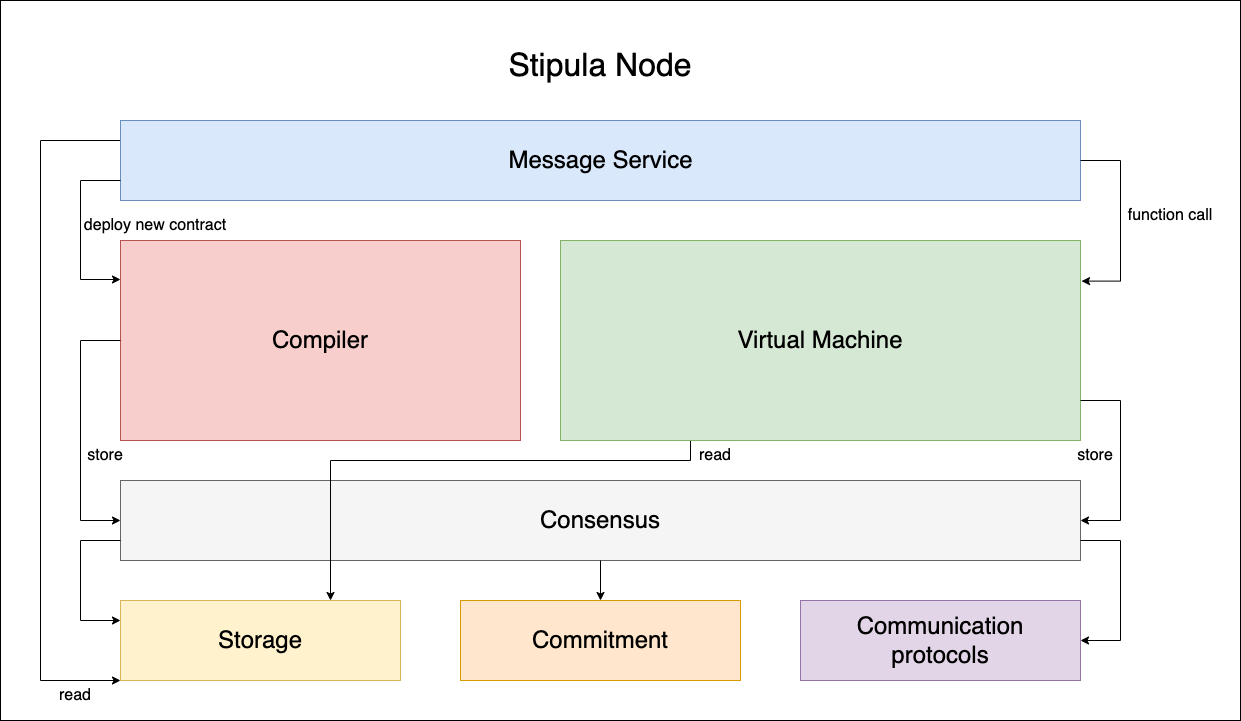
\includegraphics[height=7cm]{immagini/capitolo-4/complete-architecture.png}
		\caption{Complete architecture of all modules and interactions between them.}
		\label{fig:complete-architecture}
	\end{center}
\end{figure}

\newpage
\subsection{Message Service}

This module performs the role of \textit{server}, that is, it waits for new connections from clients. It was 
decided to use a TCP connection instead of HTTP for the following reasons:
\begin{enumerate}
	\item In order to communicate via the HTTP protocol, a \textit{web server} must be added to the 
	implementation. This would have weighed down the implementation and would not have made use of all the 
	features offered by the HTTP protocol;
	\item The TCP protocol is a \textit{reliable} and \textit{connection-oriented} protocol, that is, it frees 
	the application from the task of handling out-of-order or missing packets;
	\item The TCP protocol allows you to send and receive streams of bytes directly, instead of streams of 
	characters as is the case with the HTTP protocol. By doing so, you also get an advantage in terms of 
	efficiency.
\end{enumerate}

Once a new connection has been received from a client, the management of communication with that client is 
delegated to a \textit{thread}, in order to free up the server thread to accept new requests. Once the 
message sent by the client has been received and decoded, we proceed to check the \textit{signatures} of 
the message itself. Every message that is sent must be signed with the private key held by the client. If 
the signature check passes, then the request will be routed to other modules. The connection with the client 
remains open until the module to which the request was directed returns a response; once the response is 
received, it is sent to the client and the connection is closed.

\subsection{Compiler}

A \href[]{https://github.com/stipula-language/stipula}{first implementation} of the \textit{Stipula} language 
has been done previously. In this implementation, the language is \textit{interpreted} at \textit{runtime} 
and is executed locally on the machine. This approach has limitations if you want to translate it into the 
distributed context. Interpretation has the advantage of directly executing the code, without performing 
intermediate compilation steps. However, it has major drawbacks:
\begin{enumerate}
	\item \textit{Slow to execute}: the code is translated directly into machine code. An intermediate 
	compilation step could have optimized the code before running it;
	\item \textit{Low performance}: since the code is not optimized for the platform on which it runs;
	\item \textit{Less error checking}: this represents one of the weakest points of this approach, 
	particularly in the context of writing and executing contracts that have legal value.
\end{enumerate}
	
To overcome the limitations of this first implementation, it was decided to divide the process of executing a 
contract into two main steps:
\begin{enumerate}
	\item \textit{Compilation}: having received the contract as input, it is compiled in an intermediate 
	language called \textit{Stipula bytecode}. The characteristics of this language will be extensively 
	discussed in the following chapter;
	\item \textit{Execution}: having received the contract compiled in bytecode as input, this is executed.
\end{enumerate}

In this way we obtain an optimization in terms of performance, that is, once the contract has been compiled, 
the same contract can be called numerous times, without having to re-compile each time. Furthermore, having 
an intermediate compilation step it is possible to perform \textit{static} checks: it is possible to verify 
whether the contract states can actually be reached during execution, check if the asset transfers have been 
defined correctly and implement checks about the types of variables. As regards this last point, the 
\textit{Stipula} language is a \textit{weakly typed} language: when writing a contract it is possible to 
specify whether a variable is a \verb|asset| or is a \verb|field|. Obviously, if a variable is defined as 
\verb|field| it is necessary to perform a \textit{inference} operation to determine the specific type. 
However, it's not always possible to determine the type of a variable at compile time, so you need to 
determine it at runtime. 

The use of the bytecode language also allows you to obtain an advantage from the point of view of 
\textit{interoperability}. In fact, further compilers could be developed, which from other smart contract 
languages (i.e., Solidity), translate the smart contracts into \textit{Stipula bytecode} language.

\subsection{Virtual Machine}

The compilation phase produces code written in a particular language, specifically defined for the purpose 
of the project. Therefore, you need to build an environment for executing the contract bytecode. For this 
reason a \textit{virtual machine} has been developed. The benefits that follow from virtualization are:
\begin{enumerate}
	\item \textit{Platform independence}: the virtual machine creates an abstraction layer between the code 
	and the underlying hardware, thus allowing the code to be executed on different platforms, without the 
	need to recompile it every time;
	\item \textit{Secure environment}: the virtual machine creates a secure environment for execution, 
	especially needed for asset transfer.
\end{enumerate}

\label{stack-based-vm}
The virtual machine implemented is a \textit{stack-based virtual machine}, that is, the program variables 
are loaded onto a stack and the language instructions operate on that stack by removing or adding elements 
to the stack. A stack-based virtual machine is simpler to implement and requires fewer instructions to 
perform the same operations compared to a \textit{register-based} virtual machine. However, it must be 
taken into consideration that a stack-based virtual machine is less performing than a register-based 
virtual machine and also requires many more memory accesses. Aware of these differences, due to issues of 
time and complexity, it was decided to create a stack-based virtual machine.

The virtual machine manages various memory areas, as it must take into account the internal variables of 
the functions, the parameters of the functions and the global variables. In addition to these, there are 
also other memory areas whose purposes will be defined in the next chapter.

This module also takes care of managing the \textit{obligations}, that is, scheduling the events that will 
allow you to execute a specific portion of code, at a specific time. The management of this functionality 
involves both the compiler, in recognizing the obligation encoded in the code, and the virtual machine: 
during the execution of the contract, the scheduling request of an obligation is managed ad-hoc by a 
specific component of the virtual machine.

\subsection{Consensus}

Consensus is an essential component for the proper functioning of peer-to-peer networks, as it allows 
multiple nodes to agree on a single \textit{result}, even in the presence of failures. Without consensus, 
peer-to-peer networks would be prone to conflicts, inconsistencies, and vulnerabilities, making them less 
reliable and less secure. In a distributed context, multiple nodes work together to perform a task and 
must communicate with each other to exchange information and coordinate their actions. However, due to 
factors such as network delays, failures and communication errors, different nodes may have different 
views of system status (such as a contract or a transfer) or may produce conflicting results. In 
particular, the goals of consensus algorithms must guarantee:
\begin{enumerate}
	\item \textbf{Data consistency}: in a distributed ledger, multiple nodes can contain different copies of 
	the same data. Consensus algorithms ensure that nodes agree on a single version of the data, ensuring 
	data consistency and avoiding data corruption;
	\item \textbf{Fault tolerance}: nodes can fail or become unresponsive. The consent algorithms allow the 
	system to continue to operate even in the presence of node failures;
	\item \textbf{Conflict-free}: consensus algorithms ensure that the system is conflict-free, ensuring that 
	nodes agree on a single result;
	\item \textbf{Security}: Consensus algorithms can help prevent malicious actors from manipulating the 
	system by ensuring that all nodes agree on a single decision value, even in the presence of attacks such 
	as data tampering or \textit{Denial-of-Service} (\textit{DoS}).
\end{enumerate}

Therefore, the evolution of the status of a contract or the successful transfer of a certain amount of 
assets towards an address must be in agreement with the other nodes making up the network.

\subsection{Storage}
\label{storage-module}

This module takes care of storing various information regarding assets and contracts. In particular, 
information concerning:
\begin{enumerate}
	\item \textbf{Asset}: it is necessary to memorize information that characterizes the asset itself, such 
	as the name, a unique identifier, the total \textit{supply} and whether the asset is divisible or not. 
	Total supply is the total amount of asset that will be available for a specific asset;
	\item \textbf{Transfer of assets}: it is necessary to trace the movements of assets that are carried out 
	by customers and contracts. Later it will be explained in detail how asset transfers occur in the current 
	implementation;
	\item \textbf{Contracts}: the new contracts are loaded into a \textit{Stipula server} or a 
	\textit{Stipula node} and stored together with the bytecode produced by the compilation phase. Once a 
	contract is uploaded, it is no longer possible to make any changes;
	\item \textbf{Contract instances}: when you want to execute a contract, a new \textit{contract instance} 
	is created. The storage keeps track of \textit{each running contract instance}, together with its 
	\textit{current state}. For instance, two actors, Alice and Bob, want to activate an instance of BikeRental 
	with ItalyRent (see section \ref{bike-rental-example-definition}). There can be a BikeRental between Alice 
	and ItalyRent in state \verb|@Using|, and a BikeRental between Bob and ItalyRent in state \verb|@Return|.
\end{enumerate}

\subsection{Commitment}
\label{commitment-module}

For the context created by the proposed implementation, the commitment module represents the level at which 
information can be securely stored. Indeed, the purpose of this component is to offer a high level of security 
for the recording of information. It is not necessary to memorize all the information that is saved in the 
\textit{Storage} module, but a \textit{minimal} set of key information allows to reconstruct the evolution of 
the contract and of the asset transfers that have taken place over time. Thus, the commitment module is used to 
\textit{timestamping} the information, proving the \textit{existence} of a particular piece of information. The 
presence of this module within the implementation is not strictly necessary for the functioning of a 
\textit{Stipula} server or node, but it allows it to offer a higher level of security. As an example: we can 
devise a simple client-server implementation where the storage in managed by the server as an internal database, 
or a richer implementation where the server commits to a blockchain part of the storage to notarize the main 
info of the contract execution.

\subsection{Communication protocols}
\label{communication-protocols-module}

In a distributed context, it is necessary that the various nodes can communicate with each other to exchange 
information. The type of information exchanged can be divided into:
\begin{enumerate}
	\item Information to determine \textit{consent} about the status of a contract;
	\item Information to manage \textit{connections} with other nodes (i.e., discovery of new nodes, notify 
	that a node is congested, \dots).
\end{enumerate}

The design of a communication protocol is critical because it determines how efficiently and accurately 
information is transmitted and received. Poorly designed protocols can cause a variety of problems, such as 
slow performance, lost or corrupted data, security vulnerabilities, and difficulties in scalability and 
maintainability.

\section{Interaction between modules}

In this section we want to explain how the interactions between the various modules of the architecture take 
place. Each request sent by a client is received by the \textit{Message Service} module, which, after 
carrying out the appropriate checks, can direct the request towards different modules according to the 
specific request:
\begin{enumerate}
	\item Towards the \textit{Compiler}: when the request received represents the user's will to load a new 
	contract. The contract is received from this module, which proceeds with the compilation of the same;
	\item Towards the \textit{Virtual Machine}: when with this request the client wants to create a new 
	instance or perform a function of a specific contract instance.
	\item Towards the \textit{Storage}: when the client's request consists in a reading of some information 
	(i.e., available assets associated with its address).
\end{enumerate}

It is necessary to specify that all the requests that are addressed to the \textit{Storage} module are 
always read requests and never write requests; writing information can only be done for compiling a new 
contract (\textit{Compiler}) or for running an instance of a contract (\textit{Virtual Machine}).

If the request is of type ($1$) or of type ($2$), the results produced by the respective modules are routed 
to the consent module. The reason is that before writing any information to the storage and/or commitment 
layer, the network must agree on the same information to be written. Consequently, this phase also involves 
the module that implements all the communication protocols between the nodes, since, in order to be able to 
determine consensus within the network, the nodes must be able to communicate with each other. Furthermore, 
this module will carry out activities regardless of the requests received from the clients, in fact within 
this part of software there are also the protocols that allow you to manage the connections with the other 
nodes.

\section{Asset management}

The language offers primitives that allow you to handle the transfer of assets carefully and independently 
of how the assets are actually implemented. These design choices made the language very clear to write and 
read code.

\subsection{Definition of assets}
\label{asset-definition}

One of the most important points of the development of this thesis project concerns the provision of an 
implementation of the concept of \textit{asset}. As a basic idea, it was decided to try to reproduce the 
same characteristics of blockchain \textit{token} such as \textit{Ethereum} or \textit{Algorand}, adapting 
the complexity to the current development of the project. Thus, the main characteristics of an asset are:
\begin{enumerate}
	\item \textbf{Unique identifier}: consists of an alphanumeric string to uniquely refer to an asset;
	\item \textbf{Name of the asset}: a name is defined that can be easily remembered by a person;
	\item \textbf{Unit name}: corresponds to what is a \textit{ticker} of a company listed on the stock 
	exchange (i.e., APPL for Apple company);
	\item \textbf{Decimals}: indicates how many parts a single unit can consist of;
	\item \textbf{Maximum supply}: indicates the maximum amount of assets that can exist over time. The 
	maximum quantity also includes decimal values, for example: if you want to define an asset 
	\verb|StipulaCoin| which can only have 10 units and each unit can be divided into 100 sub-units, therefore 
	the maximum supply will be 1000 sub-units.
\end{enumerate}
Example of definition of an hypothetical \verb|StipulaCoin| asset:
\label{definition-fungible-asset}
\begin{enumerate}
	\item \textit{Unique identifier}: \verb|stipula_coin_asd345|
	\item \textit{Name of the asset}: \verb|StipulaCoin|
	\item \textit{Unit name}: \verb|STC|
	\item \textit{Decimals}: 3
	\item \textit{Maximum supply}: 1000
\end{enumerate}
The \verb|StipulaCoin| asset thus defined has an identifier (\verb|stipula_coin_asd345|), a unit name 
(\verb|STC|), has a maximum supply of 1000 sub-units and the number of decimals is equal to 3, so a single 
unit can be divided into 100 sub-units.

With this structure it is possible to define different types of assets, such as:
\begin{enumerate}
	\item \textbf{Fungible assets} (i.e., bitcoins and banknotes): an asset is fungible when it is 
	\textit{interchangeable} from the point of view of the units that compose it, i.e., that each of its units 
	is \textit{indistinguishable} the from each other, for the same nominal value. It is possible to define 
	both divisible and non-divisible fungible assets;
	\item \textbf{Non-fungible assets} (i.e., NFT): contrary to fungibility, the units that make up the asset 
	are unique and therefore are not interchangeable with each other. Furthermore, another feature that 
	distinguishes them from fungible assets is that they are not divisible.
\end{enumerate}

An example of a fungible asset was shown above (\ref{definition-fungible-asset}). An example of a 
non-fungible asset is provided:
\begin{enumerate}
	\item \textit{Unique identifier}: \verb|stipula_nft_abc123|
	\item \textit{Name of the asset}: \verb|StipulaNFT|
	\item \textit{Unit name}: \verb|SNFT|
	\item \textit{Decimals}: 0
	\item \textit{Maximum supply}: 1
\end{enumerate}
The \verb|StipulaNFT| asset thus defined has an identifier (\verb|stipula_nft_abc123|), a unit name 
(\verb|SNFT|), has a maximum supply of 1 unit and the number of decimals is equal to 0, because a 
non-fungible asset cannot be split.

However, the definition of the characteristics of an asset is not sufficient to also define in which 
\textit{way} the assets are transferred. Therefore in the next section we will proceed to provide a 
possible solution for asset transfer.

\subsection{Transfer of assets}

The way in which the transfer of assets is implemented represents one of the most delicate points of the 
whole project. When you want to send a certain amount of a specific asset, you want to guarantee some 
properties:
\begin{enumerate}
	\item \textbf{Atomicity}: the transaction must take place atomically from the sender to the recipient;
	\item \textbf{Consistency in the quantity transferred}: we want to ensure that no quantities of assets 
	are lost or quantities of assets are generated out of nothing, during a transaction;
	\item \textbf{Prevent assets from getting stuck}: you want to prevent assets from getting stuck in 
	contracts, and therefore cannot be spent;
	\item \textbf{Proof of possession}: you want to have proof that the amount of assets you want to move is 
	actually owned by the sender;
	\item \textbf{Avoid double-spending}: prevent an entity from being able to pay two recipients using 
	exactly the same amount of assets. This is a problem that does not arise with, for example, banknotes, 
	but it is a problem that affects digital assets. This problem is due to the fact that in the digital 
	context, unlike the real world, it is difficult to reproduce the concept of \textit{scarcity} of a good.
\end{enumerate}

The problems indicated in points ($1$) and ($3$) are totally solved by the \textit{Virtual Machine} 
(see section \ref{virtual-machine}), however, the check that during the transfer of assets no amount of 
assets is lost or generated, is only solved partially (see sections \ref{asset-implementation} and 
\ref{script-vm}). The solution to the other points will be explained later in sections 
\ref{asset-implementation} and \ref{virtual-machine}.

\subsubsection{Pay-to-Contract and Pay-to-Party}
\label{pay-to-contract-and-pay-to-party}

Blockchains like \textit{Ethereum} or \textit{Algorand} allow you to send and receive coins without using 
contracts and to exchange tokens using smart contracts. In the current implementation for \textit{Stipula}, 
it is not possible for two entities to exchange assets except through a contract. This is because it would 
have required the development of primitives external to the virtual machine in order to enable the transfer 
of assets without going through a contract. The purpose of the implementation is to build a platform for the 
execution of legal contracts, and not to create a platform for pure asset transaction.

Taking into account that any transfer of assets must take place through the execution of a contract, it is 
necessary to define how these transfers must take place between the participants of a contract. Each 
\textit{party} of a contract (that is, the participants of the contract) owns a pair of 
\textit{cryptographic keys}, with which it is able to send signed messages and to prove possession of 
certain properties. A party, not being able to directly send assets to another party, must send these assets 
to the contract. This operation is defined as \textbf{Pay-to-Contract} or \textbf{deposit}, i.e., when the 
party makes a function call that requires sending a certain amount of assets, it sends it to the contract. 
In the execution phase of the function call, all the necessary checks will be performed to verify that the 
party is actually the owner of that amount of assets. Once the checks have been carried out, it will now be 
the contract that guarantees the integrity of the assets, i.e., thanks to the definition of the language 
primitives, it will be the contract that ensures that no quantities of assets will be lost into thin air or 
quantities of assets will be generated from nothing . Instead, the operation that occurs when the contract 
has to send assets to a party is called \textbf{Pay-to-Party} or \textbf{withdrawal}. Again, the language 
primitives will ensure that the party will receive the correct amount of assets. Thus defining the deposit 
of assets in a contract and the withdrawal of assets from a contract, it is possible to transfer assets 
between two or more parties by means of a contract, without the need to implement additional primitives 
external to the language and specific to the implementation of the architecture. A simple example that 
illustrates how \textit{Pay-to-Contract} and \textit{Pay-to-Party} work is shown in the example in section 
\ref{asset-swap}, where two actors, Alice and Bob, exchange two assets with each other.

\subsubsection{Single-use-seals}
\label{single-use-seal-definition}

Despite the definition of an asset management structure and the definition of the operations to send and 
receive assets, the definition of a model to represent and manage the balances of various assets that a 
party can have is missing. The simplest model to implement is the \textbf{account-balance-based} model, 
where each address has a balance associated with it. With each transaction, the balance of the sent asset is 
updated, both for the sender and for the recipient. An example of an account-balance-based model:
\begin{Verbatim}[numbers=left,xleftmargin=2cm]
	...
	"partyA": {
		"asset1": {
			"balance": 123.65
		},
		"asset2": {
			"balance": 18.44
		}
	}
	...
\end{Verbatim}

However, this simple model has problems in terms of:
\begin{enumerate}
	\item \textit{Scalability}: if you want to send two transactions of an asset \verb|asset1|, these 
	transactions cannot be parallelized, as the second transaction must wait for the balance of asset 
	\verb|asset1| is updated for the sender and the recipient after the execution of the first transaction;
	\item \textit{Privacy}: it is a model that allows you to very easily track the funds associated with an 
	address.
\end{enumerate}

An alternative model has been introduced by Bitcoin: the \textbf{Unspent Transaction Output} (\textbf{UTXO}) 
model. It is a more complex model than the previous one but offers advantages in terms of scalability, 
privacy and security. To give a concrete example, we can define a UTXO as a box that contains a certain 
amount of an asset. This box is closed by a \textit{single-use-seal} which can only be broken by the owner 
of the quantity of assets in question. To explain how this model works, we introduce the following example: 
suppose Alice has to give Bob 1 \verb|StipulaCoin|. Alice owns two UTXOs, \verb|UTXO_1| and \verb|UTXO_2|, 
each of 1 \verb|StipulaCoin|. At this point, Alice chooses to use \verb|UTXO_1|, she breaks the seal and 
creates a new seal so that only Bob can then break it in turn. By doing so, \verb|UTXO_1| it becomes Bob's 
property and only he can spend it in future transactions. The breaking of the seal can only be done if the 
user is able to provide cryptographic proof that he is the rightful owner of the UTXO. The balance of Alice 
and Bob's \textbf{wallets} are given by the sum of the UTXOs in their possession: before the transaction, 
Alice had 2 \verb|StipulaCoin| contained in two different UTXOs, that is, \textit{two transaction outputs 
(received) not (yet) spent}, while Bob had 0 \verb|StipulaCoin|; after the transaction, Alice has 1 
\verb|StipulaCoin| and Bob has 1 \verb|StipulaCoin| (the one received from Alice), that is, both have 
\textit{an output of a transaction (received) not (yet) spent}.

The advantages of using this model are:
\begin{enumerate}
	\item \textit{Parallelization}\label{utxo-parallelization}: unlike the account-balance-based model, 
	transactions that correspond to two payments using two different UTXOs can be parallelized, without having 
	to wait for the balance to be updated of the transacted asset after the first transaction. Taking the 
	above example, Alice could send \verb|UTXO_1| to Bob with a transaction and send \verb|UTXO_2| at the same 
	time Charlie;
	\item Partially solves the \textit{double-spending} problem: a specific UTXO can be spent on only one 
	transaction and not on others. The problem is partially solved because the network of nodes still has to 
	verify that a user does not try to pay multiple transactions with the same UTXO;
	\item \textit{Security}: in order to spend funds, cryptographic proof of ownership of the assets to be 
	moved must be provided;
	\item \textit{Privacy}: this model encourages not to reuse the same addresses, making it more difficult 
	to trace funds. In fact, each transaction accepts UTXO as input and generates new UTXO as output. If the 
	same address is used over and over again to make payments, it becomes easier for an observer to track the 
	history of transactions associated with that address, potentially revealing sensitive information;
	\item \textbf{UTXO selection}\label{coin-selection}: consists of the process of choosing the UTXOs, from 
	the set of available UTXOs, to cover the transaction amount while minimizing the transaction fees in 
	Bitcoin. If you select UTXOs with a large value, you may pay higher transaction fees than if you selected 
	UTXOs with a smaller value. Also, if you select too many UTXOs to cover your transaction amount, you may 
	find yourself having a larger transaction size, which can also result in higher fees. Introduce the 
	following example to clarify the implications of this technique: suppose you want to send someone 0.5 
	\verb|StipulaCoin| and that you have several UTXOs in your wallet, including:
	\begin{itemize}
		\item 1 \verb|StipulaCoin|
		\item 0.7 \verb|StipulaCoin|
		\item 0.5 \verb|StipulaCoin|
		\item 0.2 \verb|StipulaCoin|
	\end{itemize}

If you select the UTXO from 1 \verb|StipulaCoin| to complete the transaction, you will end up paying a 
higher commission than if you selected the 0.5 UTXO \verb|StipulaCoin|. This is because the transaction 
size for the UTXO is 1 \verb|StipulaCoin| is greater than that of the 0.5 \verb|StipulaCoin| UTXO, which 
means that it will cost more to include in a block. Therefore, selecting the appropriate UTXOs for a 
transaction is important to minimize fees and ensure that the transaction is processed quickly and 
efficiently.
\end{enumerate}

For the implementation of the \textit{Stipula} language, it was decided to pay greater attention to network 
security (avoiding double-spending), user security (verifying ownership of funds through cryptography) and 
privacy. Hence, it was decided to implement a model similar to that of Bitcoin. The implemented 
model representation is much simpler than that of a UTXO, therefore to keep separate the original concept 
from the one implemented for the thesis, it was decided to use a different name: \textbf{single-use-seal}. 
This term wants to refer in particular to the key action that occurs during a transaction, i.e. the breaking 
of the seal by the sender and the creation of a new seal that only the recipient will be able to break in 
turn. This step represents the \textit{transfer of ownership} of a certain amount of assets from one user to 
another.

\subsubsection{Script}
\label{script-language}

The \textit{smart contract} concept was first proposed by cryptographer Nick Szabo 
\autocite{site:smart-contract-szabo}. Szabo described smart contracts as computer protocols that facilitate, 
verify, or enforce the negotiation or performance of contractual obligations, without the need for a trusted 
third party. However, it was only with the development of blockchains that smart contracts became practical to 
implement. The first blockchain-based platform where it was possible to create and execute smart contracts was 
Ethereum. This blockchain introduced a programming language called \textit{Solidity}, which allows developers 
to write smart contracts and deploy them on the blockchain.

Before Ethereum, the first large-scale application of the smart contract concept was Bitcoin with the 
implementation of the \textbf{Script} language. It is a \textit{stack-based} language and offers a flexible 
and secure way to define the conditions under which a transaction can be spent in the Bitcoin network, 
enabling more advanced transaction types, such as requiring more signatures or a certain amount of time 
before that the funds can be transferred. These rules can be combined in different ways to create more 
complex transaction types and smart contracts. For example, a transaction with multiple signatures might 
require approval from multiple parties before funds can be transferred, while a time-locked transaction 
might require a certain amount of time before funds can be accessed.

In the previous section we introduced \textit{UTXO} and its simplified version, \textit{single-use-seals}. 
When a user has to pay for a contract, he has to provide cryptographic proof of ownership of the 
single-use-seal. The naive solution is to send a message representing the call of a function, within which 
the cryptographic demonstration is provided. The cryptographic proof can consist in signing the 
single-use-seal identifier with the private key, so that the user can prove possession of it. However, 
this solution is very limited: if you wanted to implement a payment that requires approval from different 
users, you would have to update the message format or create a new message type (i.e., update the 
\verb|FunctionCall| message in order to collect more signatures). To avoid having to create many different 
message formats, it is possible to encode the cryptographic proof as a contract written in \textit{Script}. 
By doing so, the cryptographic proof can be represented by a complex contract written in \textit{Script} 
and which will be validated to verify if:
\begin{enumerate}
	\item The program is syntactically and semantically correct, and
	\item The signatures collected are correct and the conditions imposed by the contract have been respected.
\end{enumerate}

Szabo's smart contract idea is different from \textit{Stipula}'s legal contracts. \textit{Script} allows you 
to manage the expenditure of funds in a secure and advanced way, \textit{Stipula} takes care of executing 
programs that codify specific contractual obligations. The two languages have two different purposes and 
therefore can coexist in the same implementation. In fact, a language similar to \textit{Script} was used 
to manage asset transfers and whose programs are executed by a specific component of the virtual machine. 
Thus, the \textit{Virtual Machine} module allows both to execute contracts in \textit{Stipula} and contracts 
in \textit{Script}. By analogy with the language used in Bitcoin, it was decided not to change the name of 
this language, as they share the same instructions and mechanisms. All the details of how the 
\textit{Script} language works will be described later.

\subsubsection{Fungibility of assets and non-fungibility of single-use-seals}

In the \ref{asset-definition} section, the difference between fungibility and non-fungibility has been 
defined. It should be noted that a UTXO or single-use-seal \textit{is not fungible}. This is a property that 
both UTXO and single-use-seals have in common, so during the explanation we will refer to UTXO for the sake 
of brevity. A UTXO is non-fungible as it represents the value (quantity of assets) of a specific output 
obtained from a specific transaction. Once a UTXO is spent in a transaction, this UTXO is \textit{consumed}, 
and therefore can not \textit{never} be used again for a future payment. Also, a UTXO cannot be split, that 
is, you cannot break the seal, take a fraction of the amount of assets it contains, and put the same seal 
back on. If Alice has to send 2 \verb|StipulaCoin| to Bob but she only has a UTXO of 5 \verb|StipulaCoin|, 
the following actions will happen:
\begin{enumerate}
	\item Alice provides cryptographic proof that she owns the UTXO containing 5 \verb|StipulaCoin|, so she 
	breaks the seal for that UTXO;
	\item Alice prepares two new UTXOs: one of 2 \verb|StipulaCoin| with a seal that only Bob can break, and 
	a 3 \verb|StipulaCoin| UTXO with a seal that only Alice can break. The latter UTXO represents the 
	\textit{remainder} of a transaction. A similar situation can be encountered when using banknotes: if you have a banknote whose value exceeds that of the item you want to buy, the seller will withhold the amount equal to the value of the item and return it to the buyer the difference.
\end{enumerate}

The non-fungibility of UTXOs is important because it ensures that each transaction is recorded as a unique 
event, with a specific sender, recipient and value. This provides a high level of transparency and security, 
as it is difficult to manipulate transaction history. Also, since UTXOs cannot be reused, it reduces the 
risk of double-spending and makes it easier to track the movement of funds. However, it also means that it 
can be more difficult to make small or precise transactions, as UTXOs must be screened in their entirety.

\subsubsection{Difference from Ethereum}

When a user wants to interact with a smart contract on Ethereum, the user must authorize it to access their 
funds. By doing so, the contract will be able to spend funds in your name. This practice is called 
\textit{token allowance}. This feature represents a serious weakness regarding the security of funds. 
Indeed, there have been several cases of users approving malicious contracts with the aim of exfiltrating all 
possible funds. The philosophy which has been pursued for the implementation of the \textit{Stipula} 
language, and which has already been introduced previously, consists in giving the user full control over 
his own funds. When a user wants to make a function call of a specific \textit{Stipula} contract that 
requires the sending of a certain amount of assets, the user cryptographically proves ownership of the 
single-use-seal to be sent and transfers ownership to the contract. Now that the funds belong to the 
contract, the latter will be able to manage them adequately according to the defined rules. A contract 
\textit{Stipula} can never embezzle users' funds without their explicit permission. Obviously, this approach 
has the disadvantage for the user of having to sign several transactions if the contract requires it. 
Instead, in Ethereum, thanks to the token allowance, the smart contract can carry out several transactions, 
without having to ask the user to sign them each time. The proposed solutions are orthogonal to each other 
and it was decided to always aim to ensure a higher level of security, to the detriment of a limitation of 
the functions that can be offered.
